\documentclass{standalone}
\usepackage{tikz}


\begin{document}
\scalebox{2}{
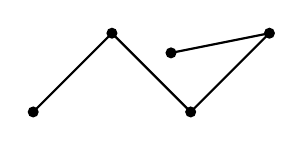
\begin{tikzpicture}[thick]
  \coordinate (a1) at (-2,0);%
  \coordinate (a2) at (-1,1);%
  \coordinate (a3) at (0,0);%
  \coordinate (a4) at (1,1);%
  \coordinate
  (a5) at (-0.25,0.75);%
  \draw (a1) -- (a2);%
  \draw (a2) -- (a3);%
  \draw (a3) -- (a4);%
  \draw (a4) -- (a5);%
  \foreach \i in {1,2,3,4,5}%
  \fill (a\i) circle (2pt);%
\end{tikzpicture}
}
\end{document}
%%% Local Variables:
%%% mode: latex
%%% TeX-master: ""
%%% End:
